\chapter{CT Frequency Response}

In this lecture we are going to focus on the frequency response and highlight it's importance in linear systems theory.

\section{Determining the frequency response (FR) of a CT system}

The frequency response of a CT LTI system can be thought of as arising in several equivalent ways. What follows is a common, but not exhaustive, list of ways the frequency response can be derived from other representations.

\subsection*{Using the Eigenvalues / Transfer Function}

Recall if we apply the Eigenfunction $e^{st}$ for the complex frequency $s \in \mathbb{C}$ as the input to a LTI system, the output is the Eigenfunction scaled by the Eigenvalue (transfer function) $H(s)$ for values of $s$ in the region of convergence, where
\[
H(s) = \int\limits_{-\infty}^{\infty} h(t) e^{-st}\; dt \; .
\]
is the bilateral Laplace transform of the impulse response.

\begin{center}
  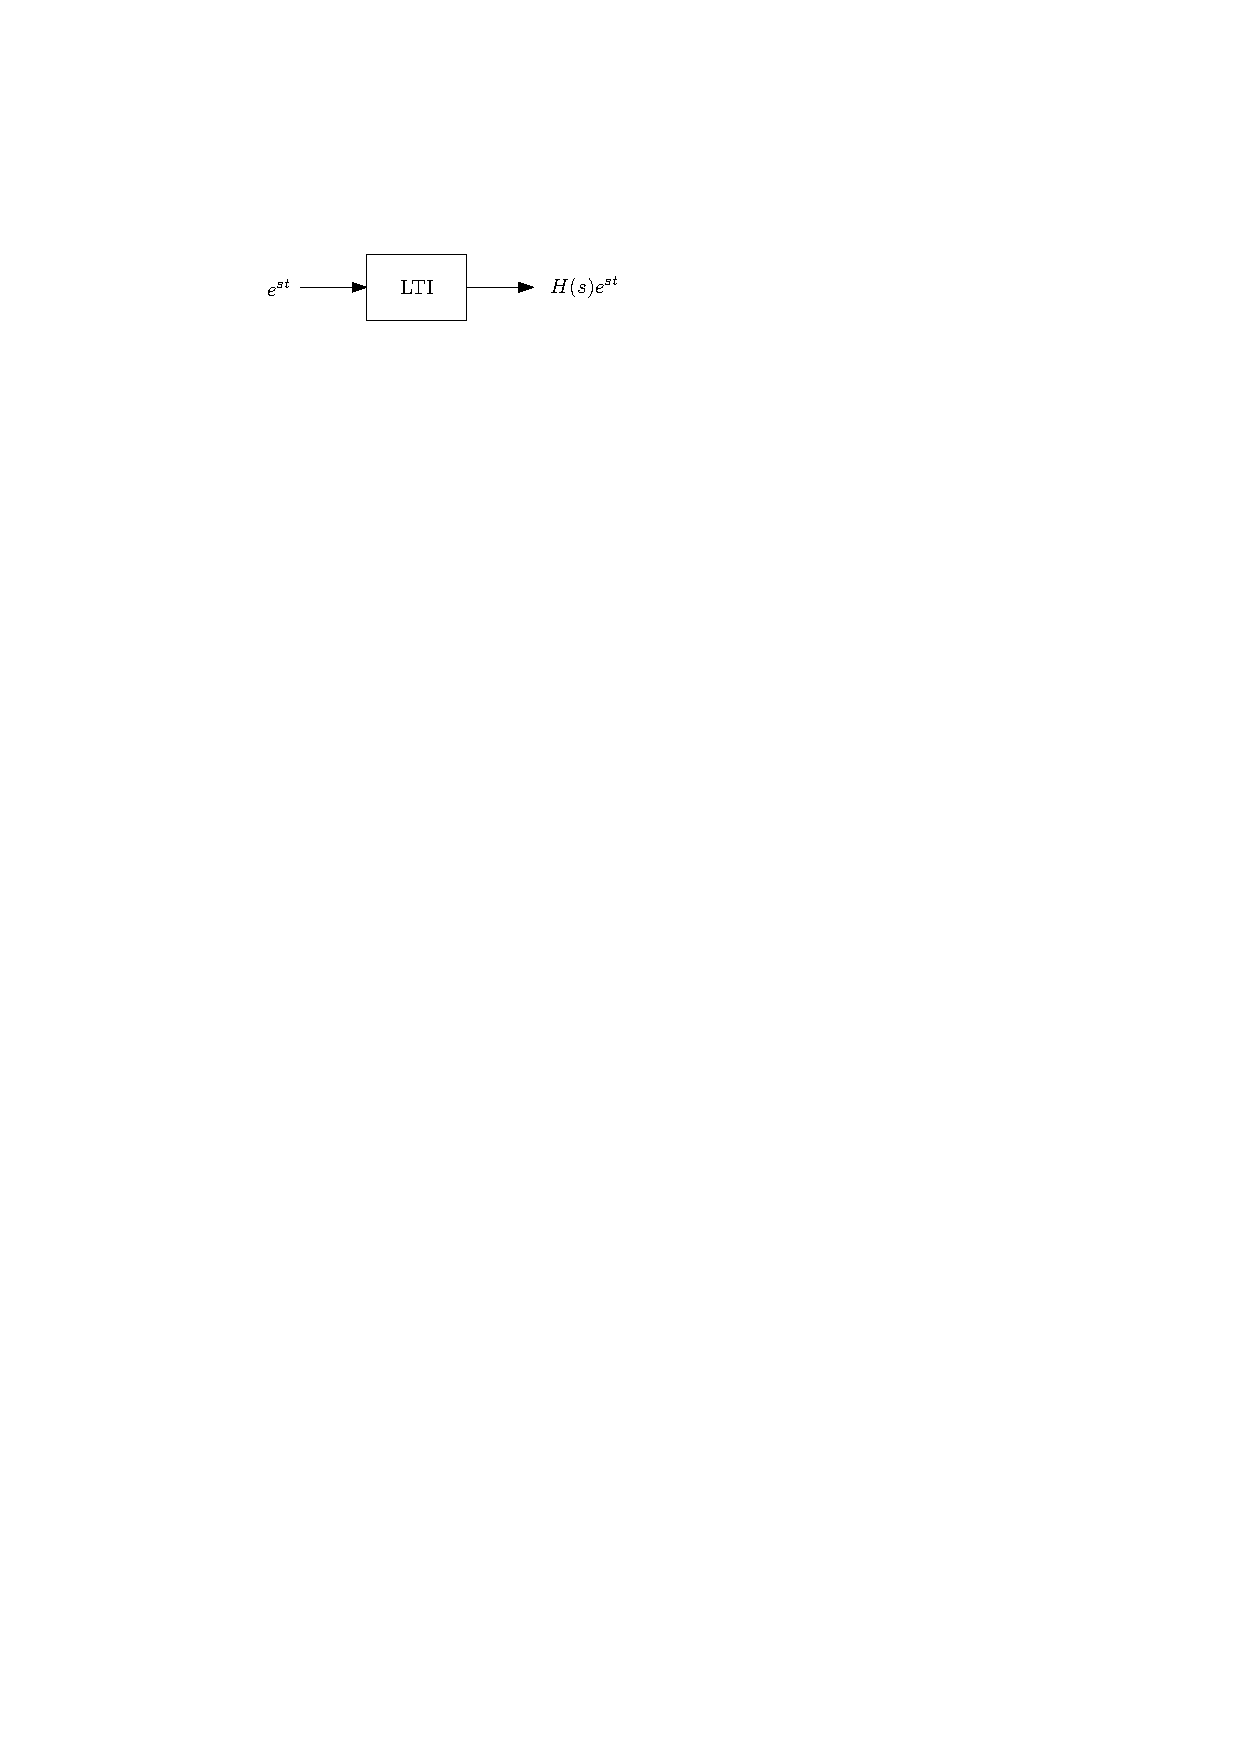
\includegraphics[scale=1]{graphics/18-ct-tf.pdf}
\end{center}

If a system is stable, then the region of convergence includes the imaginary axis $s = j\omega$. In that case, evaluating the Eigenvalues on the imaginary axis $s = j\omega$ gives the CT frequency response $H(j\omega)$. This converts from a function of a complex variable, $s$, to one of a real variable $\omega$.

\begin{example} Consider a system with Eigenvalues (transfer function)
  \[
  H(s) = \frac{2}{s+5}\mbox{ for } \Re{s} > -5
  \]
  Determine the frequency response of the system, if possible.\\

  Solution: We first need to check of the system is stable using the region-of-convergence. Since the real part of the region of convergence includes the imaginary axis ($\Re s = 0$), the system is stable. To find the frequency response we substitute $s = j\omega$ to give
  \[
  H(j\omega) = \frac{2}{j\omega+5}
  \]
  \\$\blacksquare$
\end{example}

\begin{example} Consider an apparently similar system with Eigenvalues
  \[
  H(s) = \frac{2}{s-5}\mbox{ for } \Re{s} > 5
  \]
  Determine the frequency response of the system, if possible.\\

  Solution: Again, we first need to check of the system is stable using the region-of-convergence. Since the real part of the region of convergence does not include the imaginary axis ($\Re s = 0$), the system is unstable. Thus, the frequency response does not exist.
  \\$\blacksquare$
\end{example}

\subsection*{Using the CTFT}

Another way we can view the frequency response is as the CT Fourier Transform of the impulse response. If the system is stable, then the impulse response is absolutely integrable, and the Fourier transform exists giving $H(j\omega) = \mathcal{F}\left\{h(t)\right\}$. This is connected to the transfer function by noting the bilateral Laplace transform and the Fourier Transform are identical under the substitution $s = j\omega$, which is allowed if the system is stable.

\begin{example} Suppose the impulse response of a CT LTI system is given by
  \[
  h(t) = \left(e^{-t}-e^{-6t}\right)u(t) 
  \]
  Determine the frequency response of the system, if possible.\\

  Solution: If the system is stable, the Fourier transform of the impulse response exists. Since
  \[
  \int\limits_{0}^{\infty} \left| e^{-t}-e^{-6t} \right| \; dt < \int\limits_{0}^{\infty} e^{-t} \; dt < \infty 
  \]
  the system is stable and the Fourier Transform exists, giving
  \[
H(j\omega) = \mathcal{F}\left\{ \left(e^{-t}-e^{-6t}\right)u(t) \right\} = \mathcal{F}\left\{ \left(e^{-t}u(t) \right\} - \mathcal{F}\left\{e^{-6t}\right)u(t) \right\} = \frac{1}{j\omega + 1} - \frac{1}{j\omega + 6} = \frac{7}{6-\omega^2 + j7\omega}
\]\\
$\blacksquare$
\end{example}

\subsection*{Directly from a LCCDE}

By the convolution theorem of the CTFT, the frequency response is the ratio of the output to input in the frequency domain, i.e.
\[
H(j\omega) = \frac{Y(j\omega)}{X(j\omega)}
\]
We can easily determine this ratio from the LCCDE representation of the system using the derivative property of the Fourier Transform. Recall this property states if $\mathcal{F}\{x(t)\} = X(j\omega)$ then
\[
\mathcal{F}\left\{\frac{d^n x}{dt^n}(t) \right\} = (j\omega)^n  X(j\omega) \; .
\]

If the system is stable (and thus the frequency response exists) then \textbf{all} roots of the characteriztic equation $Q(D)$ have real parts that are less than zero. If the system is stable we can take the Fourier transform of each term of the LCCDE using the derivative property, then algebrically solve for the ratio of output to input. Note this provides a signifigant savings in analysis effort since we do not have to first find the impulse response, then take it's Fourier transform to arrive at the frequency response (although that approach is still valid).

\begin{example} Consider a sytem decribed by the LCCDE
  \[
\frac{d^2y}{dt^2}(t) + 15\frac{dy}{dt}(t) + 50y(t) = 10x(t) 
  \]
  Determine the frequency response of the system, if possible.

  Solution: We first need to check for stability. The characteristic equation is $Q(D) = D^2 + 15D + 50$ which has two real roots $-10$ and $-5$. Since both are less than zero, the system is stable. Next we take the Fourier transform of both sides and apply the derivative property
  \[
  (j\omega)^2Y(j\omega) + 15(j\omega) Y(j\omega) + 50Y(j\omega) = 10X(j\omega)
  \]
  and rearrange to get the frequency response
  \[
  H(j\omega) = \frac{Y(j\omega)}{X(j\omega)} = \frac{10}{(j\omega)^2 + 15(j\omega) + 50} = \frac{10}{50-\omega^2 + j15\omega}
  \]\\
  $\blacksquare$
\end{example}

\section{Magnitude-phase representation of the CTFR}

Note that any complex valued function can be expressed in polar form using the magnitude and phase. Specifically the input and output can be put into this form
\[
X(j\omega) = |X(j\omega)|e^{\angle X(j\omega)}
\]
\[
Y(j\omega) = |Y(j\omega)|e^{\angle Y(j\omega)}
\]

By the convolution theorem then
  \[
  H(j\omega) = \frac{Y(j\omega)}{X(j\omega)} = \frac{|Y(j\omega)|e^{\angle Y(j\omega)}}{X(j\omega) = |X(j\omega)|e^{\angle X(j\omega)}} = \frac{|Y(j\omega)|}{|X(j\omega)|}e^{\angle Y(j\omega) - \angle X(j\omega)} = |H(j\omega)|e^{\angle H(j\omega)}
  \]
  Thus we see that
  \[
  |H(j\omega)| = \frac{|Y(j\omega)|}{|X(j\omega)|}
  \]
  and
  \[
  \angle H(j\omega) = \angle Y(j\omega) - \angle X(j\omega)
  \]
  This is the magnitude and phase representation of the frequency response.
  
\section{CTFR acting on sinusoids}

The advantage of the magnitude and phase representation of the frequency response, is the ease with which we can find the output due to a sinusoidal input. If we apply a sinusoidal input $x(t) = A e^{j\omega t}$, the output is a the same sinusoid scaled by the frequency response $y(t) = H(j\omega) A e^{j\omega t}$.

\begin{center}
  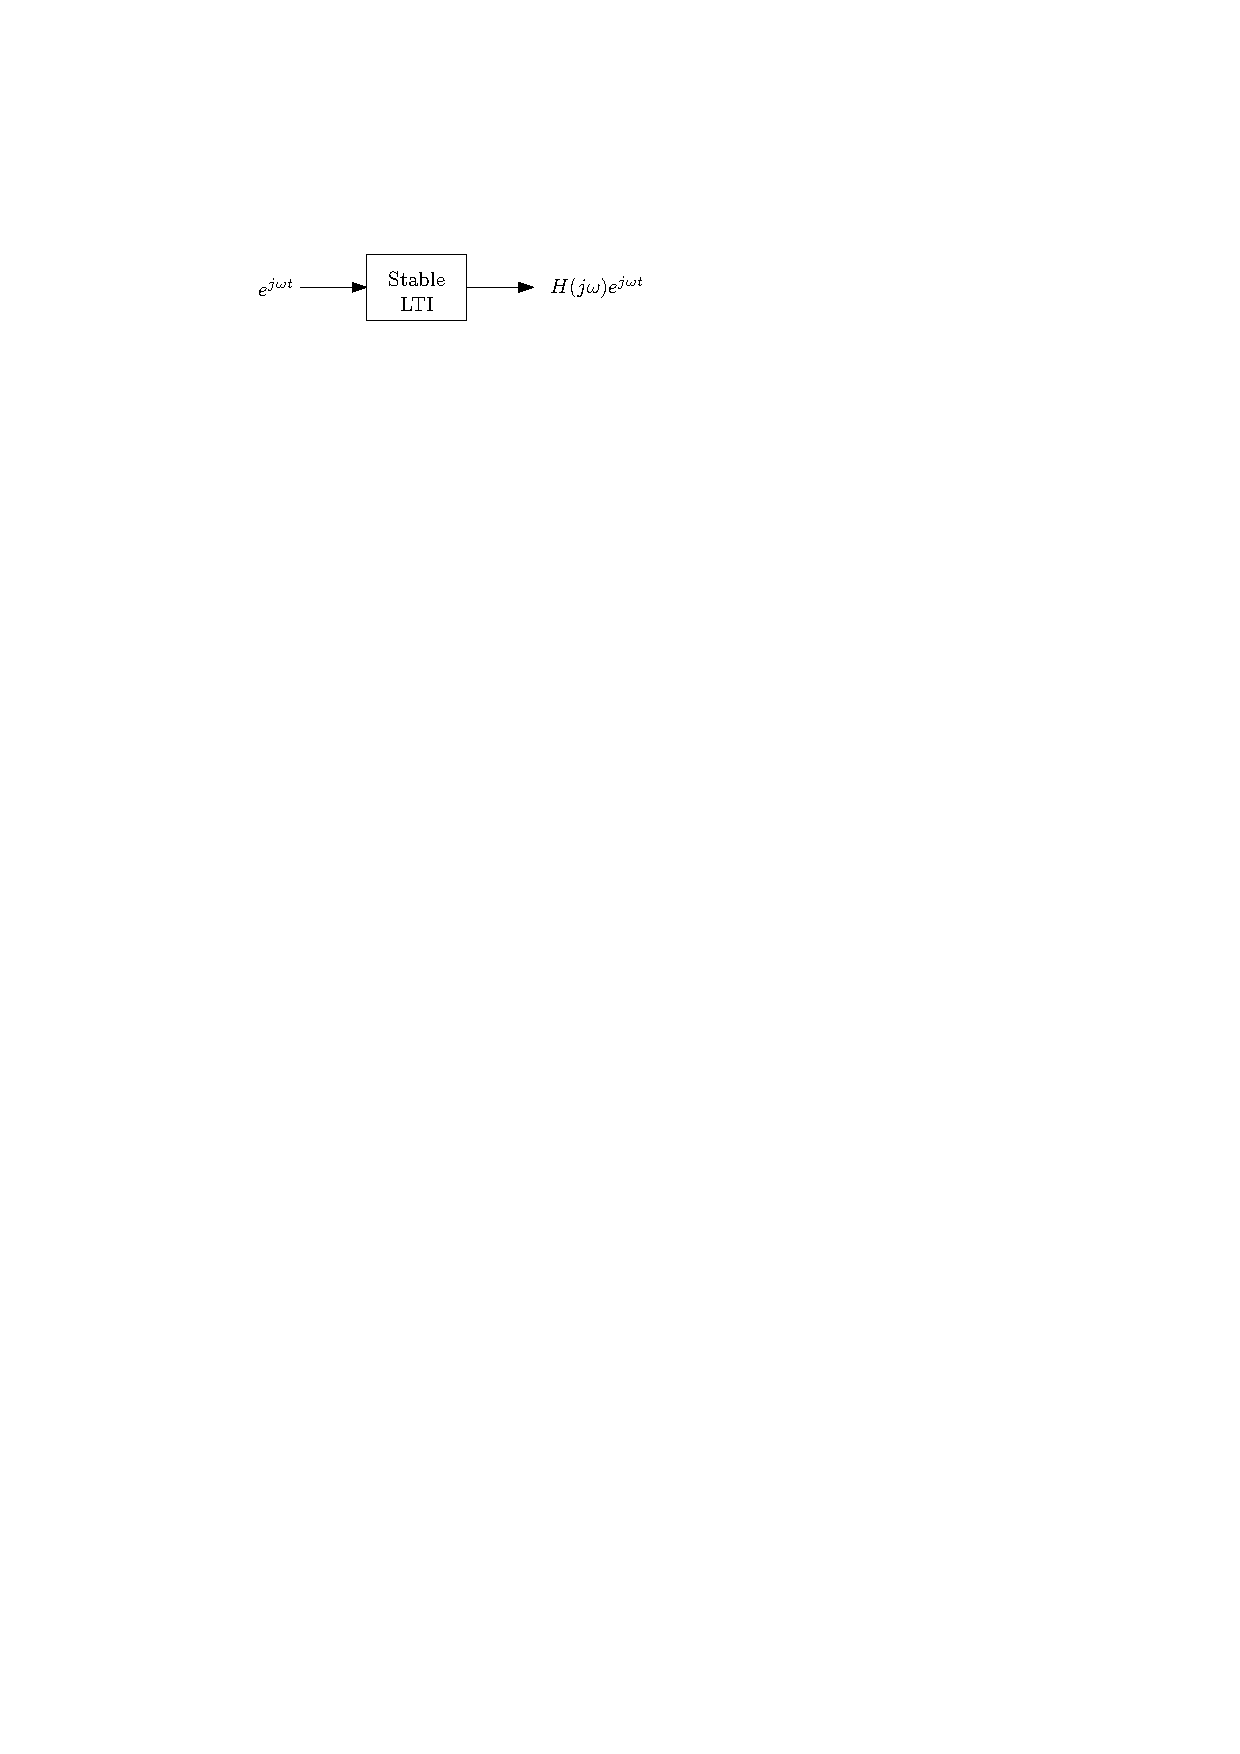
\includegraphics[scale=1]{graphics/18-ct-fr.pdf}
\end{center}

Now using the magnitude and phase representation
\[
y(t) = H(j\omega) A e^{j\omega t} = |H(j\omega)|e^{\angle H(j\omega)} A e^{j\omega t} = A |H(j\omega)| e^{j\omega t + \angle H(j\omega)} 
\]
Thus we can interpret the frequency response as telling us how the input sinsusoids are scaled in magnitude and phase shifted as they pass through the system.

By the linearity property this extends to real sinusoidal inputs since
\begin{align*}
  x(t) &\longrightarrow y(t)\\
  \sin(\omega t) &\longrightarrow \frac{1}{2j}|H(j\omega)| e^{j\omega t + \angle H(j\omega)} - \frac{1}{2j}|H(j\omega)| e^{-j\omega t + \angle H(j\omega)}\\
  \sin(\omega t) &\longrightarrow |H(j\omega)|\sin(\omega t + \angle H(j\omega))  
\end{align*}
and
\begin{align*}
  x(t) &\longrightarrow y(t)\\
  \cos(\omega t) &\longrightarrow \frac{1}{2}|H(j\omega)| e^{j\omega t + \angle H(j\omega)} + \frac{1}{2}|H(j\omega)| e^{-j\omega t + \angle H(j\omega)}\\
  \cos(\omega t) &\longrightarrow |H(j\omega)|\cos(\omega t + \angle H(j\omega))  
\end{align*}

Also by the linearity property this analysis extends to the CT Fourier representation of a signal (an infinite sum of sinusoids):
\[
x(t) = \frac{1}{2\pi}\int\limits_{-\infty}^{\infty} X(j \omega) \, e^{j \omega t}\; d\omega \;\longrightarrow\; y(t) = \frac{1}{2\pi}\int\limits_{-\infty}^{\infty} H(j \omega) X(j \omega) \, e^{j \omega t}\; d\omega = \frac{1}{2\pi}\int\limits_{-\infty}^{\infty} \left| H(j \omega)\right| X(j \omega) \, e^{j \omega t + \angle H(j \omega)}\; d\omega
\]

Thus we arrive at the reason for the name \textit{Frequency Response} -- it specifies the the response of a stable system to any linear combination of sinusoidal inputs, i.e. any signal with a Fourier Transform.


\subsection{Bode plots}

We can visualize the frequency response as a plot of the real and imaginary part, or, of the magnitude and phase. Since the magnitude and phase allow us to directly see the system behavior at a given frequency, those plots are much more useful.

Rather than simply plot the magnitude and phase as a function of $\omega$, it is common to change the abscissa (horizontal / $\omega$-axis) to be on a logarithmic scale and so only plot the positive frequency portion of the spectrum (recall if the signal is real, the frequency response is even, so no information is lost). This is because the frequency response for physically realizable systems changes slowly as a function of frequency. Plotting on a log-scale compresses this information horizontally so that we can see how a wide range of frequency content is scaled. When plotting the magnitude spectrum it is also common to make the ordinate (vertical / gain axis) to be in decibels (dB). This is because of Weber's law, which states the humans perceive a doubling in strength of stimulus, when it is actually a ten-fold increase. Thus the magnitude of the frequency response in dB is $20 \log_{10} |H(j\omega)|$. When the frequency response is plotted this particular way we get what is called a \textit{Bode plot} (after the engineer Hendrik Wade Bode, an important figure in the development of control theory).

You will likely encounter Bode plots at several points in your career, so it is important to understand them well enough to create them on your own using software and read them. Also data-sheets and other documentation for CT devices generally use a Bode plot rather than giving an explicit mathematical model of the frequency response. It is also instructive to learn how to plot them manually (which was the traditional way to do it) since it gives you insight that can help with reverse engineering a model, however we do not cover this in detail in this course. Note that we will plot the spectrum as a function of frequency in units of rad/s, but it is also common to see it plotted in units of Hz. Take care to read the horizontal axis label as mixing up the two is a common source of error.

\begin{example} Consider a frequency response given by
  \[
  H(j\omega) = \frac{20000}{(j\omega)^2 + 300(j\omega) + 20000}
  \]
  The following Matlab code shows you how to plot the spectrum as a Bode plot (with some extra code to make it look nicer). You should read the documentation for the \texttt{bode} command in Matlab. It is also easy to just compute the magnitude and phase yourself.
  
\begin{verbatim}
H = tf([20000],[1,300,20000]);
[mag,ph,w] = bode(H);

% Create a nice bode plot 
hFig = figure();
hold on;

subplot(2,1,1);
hm = semilogx(w,20*log10(squeeze(mag)));
grid on;
hTitle  = title ('Frequency Response');
hYLabel1 = ylabel('Magnitude (dB)');
set(gca, 'FontSize', 14, 'YTick', -60:10:20, ...
    'Box', 'off', 'LineWidth', 2);

subplot(2,1,2);
hp = semilogx(w,squeeze(ph*(pi/180)));
grid on;
hYLabel2 = ylabel('Phase (radians)');
hXLabel = xlabel('Frequency (rad/s)');
set(gca, 'FontSize', 14, 'Box', 'off', 'LineWidth', 2);

set(hm, 'linewidth', 2);
set(hp, 'linewidth', 2);
set([hXLabel, hYLabel1, hYLabel2]  , ...
     'FontSize'   , 14          );
set( hTitle                    , ...
     'FontSize'   , 14          , ...
     'FontWeight' , 'bold'      );
\end{verbatim}
This gives the following plot
\begin{center}
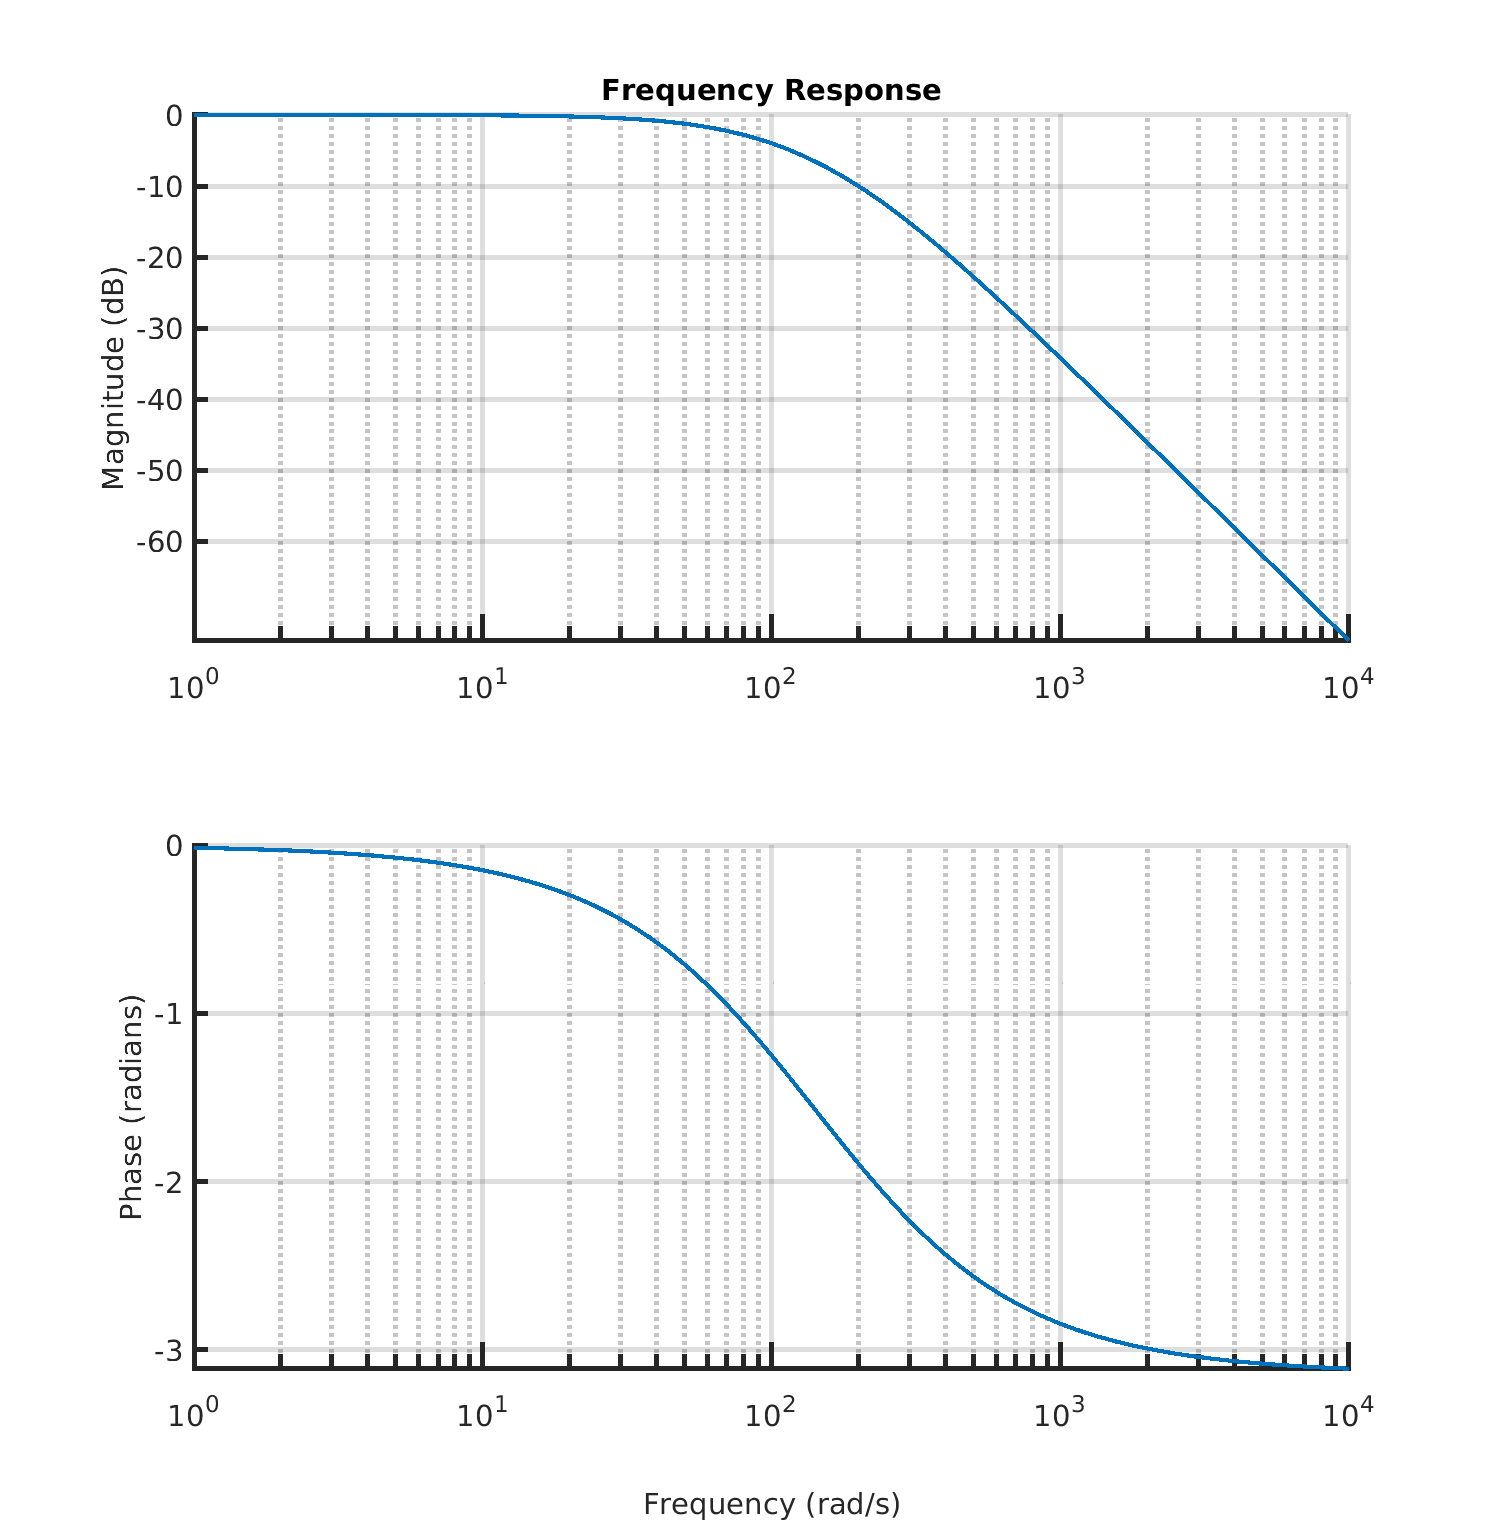
\includegraphics[scale=0.5]{graphics/lecture20_1.png}
\end{center}

$\blacksquare$
\end{example}

To read a Bode plot to see the behavior of the system at a given frequency, one need only read the values off the plot and convert from dB to a unit-less gain. A common mistake is to not realize the horizontal axis is logarithmic.

\begin{example}
  Suppose you are given the Bode plot (only) from the previous example and are asked what the output of the system is when the input is $x(t) = \cos(2\pi 32 t)$, i.e. a sinusoid at 32 Hz.\\
  \textbf{Solution:} First we determine the frequency in rad/s, $\omega = 2\pi 32 \approx 200$ rad/s. We go to that frequency on the Bode plot and read off a value of about $-10$ dB for the magnitude and about $-1.9$ rad for the phase. To convert back from dB
  \[
  |H(200)| = 10^{\frac{-10}{20}} \approx 0.3 
  \]
  so the output would be
  \[
  y(t) \approx 0.3\cos(2\pi 32 t - 1.9)
  \]
  $\blacksquare$
\end{example}

\section{CTFR of first and second order systems}

TODO
